

\section{The gem5 Simulator}

There is ``a new golden age for computer architecture''~\cite{turinglecture,cacm} driven by changes in technology (e.g., the slowdown of Moore's Law and Dennard Scaling) and ever increasing computational needs.
One of the first steps in research and development of new hardware architectures is software-based modeling and simulation.
The gem5 simulator~\cite{Binkert-gem5-2011} is currently one of the most popular academic-focused computer architecture simulation frameworks.
Since its publication in 2011, the gem5 paper has been cited over 3600 times\footnote{\url{https://scholar.google.com/scholar?q=gem5}}, and every year many papers published in the top computer architecture venues use gem5 as their main evaluation technique.

The gem5 simulator~\cite{Binkert-gem5-2011} is an open source community-supported computer architecture simulator system.
It consists of a simulator core and models for everything from out of order processors, to DRAM, to network devices.
The gem5 project consists of the gem5 simulator\footnote{\url{https://gem5.googlesource.com/public/gem5}}, documentation\footnote{\url{https://www.gem5.org/}}, and common resources\footnote{\url{https://gem5.googlesource.com/public/gem5-resources}} that enable computer architecture research.

The gem5 project is governed by a meritocratic, consensus-based community governance document\footnote{\url{https://www.gem5.org/governance/}} with a goal to provide a tool to further the state of the art in computer architecture.
The goal of gem5 is to provide a tool to further the state of the art in computer architecture. gem5 can be used for (but is not limited to) computer-architecture research, advanced development, system-level performance analysis and design-space exploration, hardware-software co-design, and low-level software performance analysis.
Another goal of gem5 is to be a common framework for computer architecture.
A common framework in the academic community makes it easier for other researchers to share workloads as well as models and to compare and contrast with other architectural techniques.

The gem5 community strives to balance the needs of its three categories of users: academic researchers, industry researchers, and students.
For instance, gem5 strives to balance adding new features (important to researchers) and a stable code base (important for students).
Specific user needs important to the community are enumerated below:
\begin{itemize}
    \item Effectively and efficiently emulate the behavior of modern processors in a way that balances simulation performance and accuracy
    \item Serve as a malleable baseline infrastructure that can easily be adapted to emulate the desired behaviors
    \item Provide a core set of APIs and features that remain relatively stable
    \item Incorporate features that make it easy for companies and research groups to stay up to date with the tip and continue contributing to the project
    \item Additionally, the gem5 community is committed to openness, transparency, and inclusiveness.
\end{itemize}

In this paper, we discuss the current state of gem5.
We first give an overview of gem5's main features available today, and then quickly discuss the past, present, and future of gem5.
Then, we include a significant section which describes the major changes in gem5 in the past nine years since the initial gem5 release.

It has taken a huge number of people to make gem5 what it is today.
One of the goals of this paper is to recognize the hard work on this community infrastructure which is often overlooked.
We have tried to include everyone who has contributed and documented all of the major changes.

\subsection{gem5's main features}

The gem5 simulator is a cycle-level computer system simulation environment.
At its core, gem5 contains an event-driven simulation engine.
On top of this simulation engine, gem5 implements a large number of models for system components from CPUs (out-of-order designs, in-order designs, and others), memories (such as DDR3/4, GDDR5, HBM, and HMC), on-chip interconnects, coherent caches, I/O devices, and many others.
The gem5 project also contains tests to help find bugs, a complex and feature rich statistics database, and a Python scripting interface to describe systems under test and run simulations.

The gem5 simulator has modular support for multiple ISAs.
gem5 currently supports Arm, GPU ISAs, MIPS, Power, RISC-V, SPARC, and x86.
These ISAs not only include the details to execute each instruction, but also the system-specific devices necessary for full system simulation.
There is robust full system support for Linux on Arm and x86 and many other ISAs have some level of full system support.

All of these ISAs can be used with any of gem5's CPU models as the CPU models are designed to be ISA-agnostic.
gem5 includes four different CPU models which span the fidelity performance continuum.
The highest performance CPU model is based on the kernel virtual machine (KVM) and leverages hardware virtualization to execute \emph{at native speeds}~\cite{full-speed-ahead}.
Although the KVM CPU model can execute at native speed, it does not model the timing of execution or memory.
gem5 also contains ``simple'' CPU models which are single-cycle models that can be used for memory system studies or other studies that do not require high-fidelity execution models.
Finally, gem5 contains a detailed in-order CPU model (the ``minor'' CPU) and an out-of-order CPU model (the ``O3'' CPU).

Underlying the memory system model in gem5 is a modular port interface which allows any component that implements the port API to be connected to any other component implementing that API.
This allows models designed for one system to be easily used in other system designs.

There are two different cache systems in gem5, Ruby which models cache coherence protocols with high fidelity, and the ``classic'' caches.
Ruby enables user-defined cache coherence protocols, though gem5 includes many protocols out of the box.
There are now 12 unique protocols including GPU-specific protocols~\cite{viper}, research protocols like token coherence~\cite{token-coherence} and region-coherence protocols~\cite{Power2012hsc}, and teaching protocols~\cite{coherence-primer}.
Users can also choose to use the detailed Garnet network mode~\cite{garnet-2} when using Ruby caches which offers cycle-level detail for the on-chip network.

The classic caches have a single hard-coded hierarchical MOESI coherence protocol.
However, this cache model is easily composable allowing users to construct hierarchical cache topologies without worrying about the correctness of the coherence protocol.
Both Ruby and the classic caches can be used with any CPU model, any ISA, and any memory controller model.

The gem5 simulator also includes an event-driven DRAM model.
This DRAM model is easily configurable with the timing parameters for a variety of different DRAM controllers including DDR3, DDR4, GDDR, HBM, HMC, LPDDR4, LPDDR5, and others.
Although this is not a cycle-accurate DRAM model like DRAMSim~\cite{} or Ramulator~\cite{}, it is nearly as accurate while providing more flexibility and higher performance~\cite{hansson-ispass-paper}

In addition to CPU models, gem5 also includes a cycle-level compute-based GPU~\cite{}.
This GPU model does not support graphics applications, but supports many compute applications based on OpenCL.
(Should probably add a couple more sentences.)

An important component to full system simulation is supporting I/O and other devices.
gem5 supports many system-agnostic devices such as disk controllers, PCI components, ethernet controllers, etc. and system-specific devices such as the Arm GIC and SMMU and x86 PC devices.
Additionally, gem5 contains support for a ``fake'' graphics GPU to enable simulating applications that depend on graphics APIs.

Finally, gem5 has been integrated with other computer architecture simulator systems to enable users with models in other simulator systems to use gem5's features.
For instance, gem5 has been integrated with the System Simulation Toolkit (SST)~\cite{} which uses gem5's detailed CPU models in conjunction with SST's multi-node modeling capabilities.
The IEEE standard SystemC API~\cite{} has also been integrated with gem5 to enable users with SystemC models to use them as gem5 components.

Although there are many computer architecture simulators, and many of these are open source with features that overlap with gem5, gem5 is a unique simulation infrastructure.
\begin{itemize}
    \item gem5 is \emph{dynamically configurable} through a robust Python-based scripting interface. Most other simulators are configured statically with flat text files (e.g., json) or at compilation time. On the other hand, gem5 allows users to simulate complex systems much more easily by using object-oriented Python scripts to compose simpler systems into more complex ones.
    \item gem5 is \emph{extensible} through a clean model API. gem5 has over XXX models and adding new models is straightforward and well documented.
    \item gem5 is a \emph{full system} simulator. Its high-fidelity models can support booting unmodified operating systems and running modified applications with cycle-level statistics.
    \item gem5 is a \emph{community-driven} and \emph{frequently updated} project. The gem5 community is thriving. Since its original release nine years ago, there have been over 250 unique contributors and over 7500 commits. Even in the last six months, gem5 has had over 850 commits and 50 unique contributors.
\end{itemize}

\subsection{The past nine years}

The gem5 simulator has been wildly successful in the past nine years since the initial release of gem5.
In this time, the use of gem5 has exploded.
Although not a perfect metric, the gem5 paper has received over 3600 citations according to Google Scholar.

At the same time, the contributor community has also grown.
Figures~\ref{fig:commits} shows the number of commits per year and Figure~\ref{fig:contributors} shows the number of unique contributors per year.
These figures show that since the initial release of gem5 in 2011, development has been significantly accelerating.

\begin{figure}
    \centering
    \subcaptionbox{Number of commits\label{fig:commits}}{
      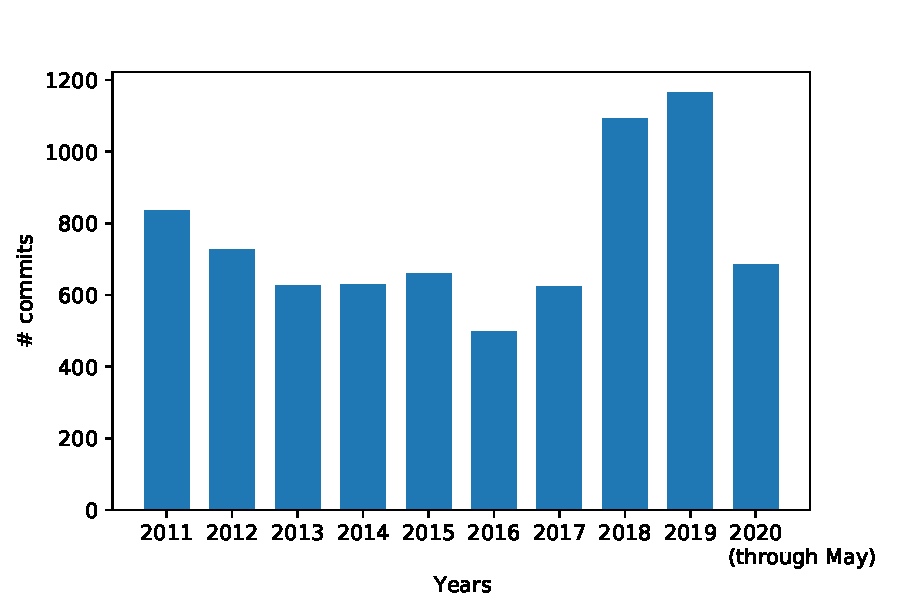
\includegraphics[height=4cm]{fig/gem5_commits.pdf}
    }
    \subcaptionbox{Number of contributors\label{fig:contributors}}{
      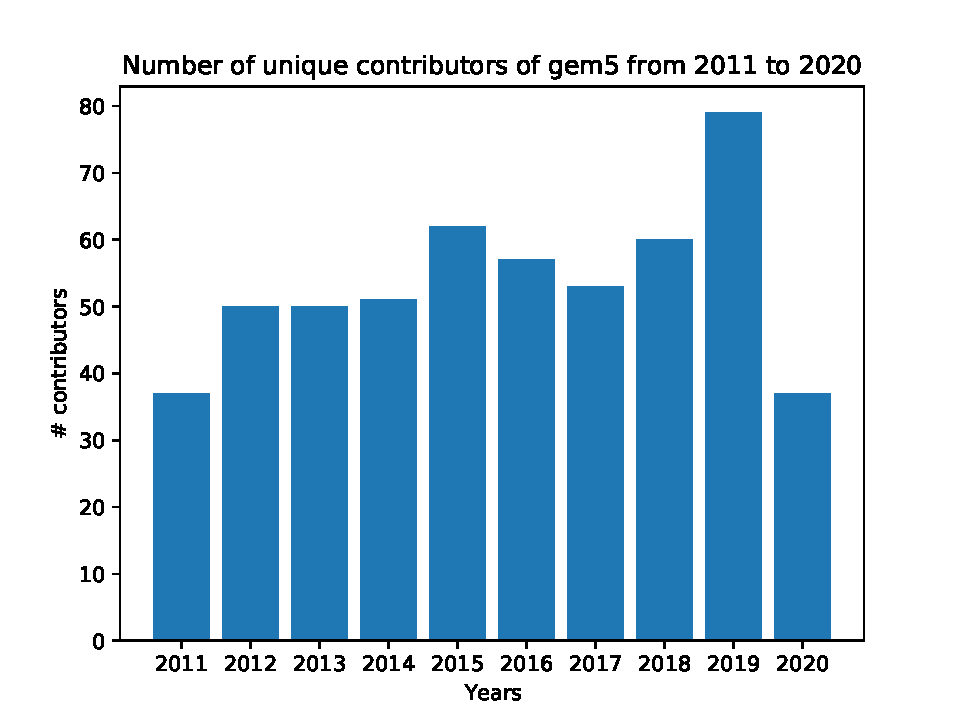
\includegraphics[height=4cm]{fig/gem5_contributors.pdf}
    }
    \caption{Number of gem5 commits and contributors from 2011 to 2020.}
    \label{fig:gem5_commits_contributors}
\end{figure}

With this acceleration in use and development of gem5 came growing pains~\cite{Power-gem5horrors-2015}.
The gem5 community was going through a shift from a small project with most contributors from one or two academic labs to a project with worldwide-distributed contributors.
Additionally, given the growing user base, we could no longer assume that all gem5 users were also going to be main developers.

\subsection{gem5 now}
\label{sec:current-gem5}

To solve these problems the gem5 community has made major changes in the past nine years.
We now have a formal governance structure, we have improved our documentation, we have moved to a better distributed development platform, and improved our community outreach.
There are still many ways we can improve (see~\ref{sec:future}), but we have already come a long way!

To solve these problems we
\begin{itemize}
    \item Instituted a governance structure
    \item Improved documentation (cite Learning gem5)
    \item Worked to fund raise to get a developer to focus on things like testing
    \item Moved development model to modern tools (git, gerrit)
    \item Created a contributing document to help people get started
\end{itemize}

\subsection{The future of gem5}
\label{sec:future}

The future of gem5 is bright.

\begin{itemize}
    \item Lots of new stuff coming in a new roadmap that's coming soon!
    \begin{itemize}
        \item Improved python interface
        \item New RAM models (including NVM)
        \item Garnet 3.0
        \item Models for ML accelerators
        \item Known-good configurations
        \item Many more.
    \end{itemize}
    \item Here, we talk about how to contribute to gem5.
    \item We will do a better job recognizing contributions. The gem5 project is only successful with the community is vibrant. We have taken positive steps towards making it easier to contribute (like a governance document and contributing documentation), but we need to do more. We will encourage everyone to contribute.
    \item More educational material coming!
    \item More workshops, tutorials, etc.
\end{itemize}
